\chapter{Healthcare Application \& Dataset}
\label{chap:Dataset}
This chapter will provide the reader with relevant information about the dataset at hand. Indeed, the idea of our approach, \emph{KG-RNN}, is quite general but we demonstrate its usefulness in a concrete application in this thesis. \\

In particular, we develop the concept of \emph{Enhanced Healthcare} and apply our technique to the diagnosis of disease at a patient discharge. To sum up the structure of chapter, we will introduce the dataset in section~\ref{sec:Description}, its source as well as its limitation and scope. Besides, we will explain the preparation procedure of the dataset in section~\ref{sec:Preparation}, how we are processing it and formatting it to be ready for modeling. Finally, we will describe and present statistics about the dataset in section~\ref{sec:Statistics} in order for the reader to have a better grasp of the big picture, the distributions and possibilities offered. \\

All of this bearing in mind our end goal: \textbf{Predict the one or multiple diagnoses assigned to a patient at discharge, among the top-50 most popular ones, given the different events occurring for this patient (measurements, medication, \dots).}

\section{Description}
\label{sec:Description}
To tackle our task of enhancing and improving healthcare by predicting diagnoses of patients at discharge of their ICU stay, we decided to utilize the MIMIC-III dataset~\footnote{\url{https://mimic.physionet.org/}}. This dataset includes over 40 thousand patients with multiple admissions per patient, making for a bit less than 60 thousand in total. All the information is de-identified and subject to restricted database, requiring going through a training program before being able to download any file. All in all, the data spans from June 2001 to October 2012. \\

As a high level, the main component of the dataset is \textit{admissions}; additionally other tables provide information about the different measurements taken throughout a patient time span as well as prescribed drugs. Finally, we are given the diagnoses at discharge, that is both diseases and procedures for the patient. \\

These diagnoses at discharge are represented in the form of ICD9 (\textit{International Classification of Diseases}) codes, which are maintained by the World Health Organization. The purpose of the system is to create a mapping between conditions and generic categories, with different levels of granularity. Indeed, this classification forms a tree where upper-level branches are including the set of similar diseases with specific variations. \\

A database of all the ICD codes for version 9 (\textit{ICD9}) can be found at~\url{http://www.icd9data.com/} and here are a few examples to get the reader acquainted with the system:

\begin{table}[H]
 \begin{center}
  \begin{tabular}{ l | p{7cm} }
   \textbf{ICD9 code or range} & \textbf{Description} \\ \hline
   001-139 & Infectious and Parasitic Diseases. \\ \hline
   010-018 & Tuberculosis. \\ \hline
   011 & Pulmonary tuberculosis. \\ \hline
   011.0 & Tuberculosis of lung infiltrative. \\ \hline
   011.03 & Tuberculosis of lung, infiltrative, tubercle bacilli found (in sputum) by microscopy. \\
   \hline
  \end{tabular}
 \end{center}
\end{table}

In the following tables, we will enumerate and describe the different fields available to our research. We filtered these fields and eventually only describe the ones we are using and that is of interest for our application at hand but many more are available in the \textit{MIMIC-III} dataset. \\

Table containing all the admissions from the different patients:

\begin{table}[H]
 \begin{center}
  \caption{Admissions}
  \begin{tabular}{| l | p{7cm} | c | }
   \hline
   \textbf{Name} & \textbf{Description} & \textbf{Example value} \\ \hline
   SUBJECT\_ID &  Unique identifier for the patient. & 23 \\ \hline
   HADM\_ID & Unique identifier for the admission. & 124321 \\ \hline
   ADMITTIME & Time at which the patient was admitted to the hospital. & 2157-10-18 19:34:00 \\ \hline
   DISCHTIME & Time at which the patient was discharged from the hospital. & 2157-10-25 14:00:00 \\ \hline
   DIAGNOSIS & Preliminary, free text diagnosis for the patient on hospital admission. & BRAIN MASS \\
   \hline
  \end{tabular}
 \end{center}
\end{table}

Table containing the different ICD9 codes diagnosed at discharge of the ICU stay:

\begin{table}[H]
 \begin{center}
  \caption{Diagnoses}
  \begin{tabular}{| l | p{7cm} | c | }
   \hline
   \textbf{Name} & \textbf{Description} & \textbf{Example value} \\ \hline
   SUBJECT\_ID &  Unique identifier for the patient. & 62641 \\ \hline
   HADM\_ID & Unique identifier for the admission. & 154460 \\ \hline
   ICD9\_CODE & Diagnoses assigned to the patient at discharge for a given admission. & 3404 \\ \hline
   SEQ\_NUM & Priority number of the given ICD9 code for the patient's admission. & 3 \\
   \hline
  \end{tabular}
 \end{center}
\end{table}

Table containing the different laboratory measurements on a patient during his stay at the ICU:

\begin{table}[H]
 \begin{center}
  \caption{Laboratory measurements}
  \begin{tabular}{| l | p{7cm} | c | }
   \hline
   \textbf{Name} & \textbf{Description} & \textbf{Example value} \\ \hline
   SUBJECT\_ID &  Unique identifier for the patient. & 3 \\ \hline
   HADM\_ID & Unique identifier for the admission. & 145834 \\ \hline
   ITEMID & Unique identifier for the measurement type in the database. & 50868 (\textit{Bicarbonate}) \\ \hline
   CHARTTIME & Time at which the observation was charted. & 2101-10-20 16:40:00 \\ \hline
   VALUENUM & Value measured for the specific measure \textit{ITEMID}. & 17.0 \\ \hline
   VALUEUOM & Unit of measurement for the measure \textit{ITEMID}. & mEq/L \\
   \hline
  \end{tabular}
 \end{center}
\end{table}

Table containing the different input fluids administered to a patient during his stay at the ICU:

\begin{table}[H]
 \begin{center}
  \caption{Input events from CareVue (Electronic Medical Records system)}
  \begin{tabular}{| l | p{7cm} | c | }
   \hline
   \textbf{Name} & \textbf{Description} & \textbf{Example value} \\ \hline
   SUBJECT\_ID &  Unique identifier for the patient. & 24457 \\ \hline
   HADM\_ID & Unique identifier for the admission. & 184834 \\ \hline
   ITEMID & Unique identifier for the fluid type in the database. & 30056 (\textit{Po Intake}) \\ \hline
   CHARTTIME & Time at which the observation was charted. & 2193-09-11 09:00:00 \\ \hline
   AMOUNT & Amount of the drug or substance administered \textit{ITEMID}. & 100.0 \\ \hline
   AMOUNTUOM & Unit of measurement of the drug or substance administered \textit{ITEMID}. & ml \\
   \hline
  \end{tabular}
 \end{center}
\end{table}

Table containing the different input fluids administered to a patient during his stay at the ICU:

\begin{table}[H]
 \begin{center}
  \caption{Input events from Metavision (Electronic Medical Records system)}
  \begin{tabular}{| l | p{7cm} | c | }
   \hline
   \textbf{Name} & \textbf{Description} & \textbf{Example value} \\ \hline
   SUBJECT\_ID &  Unique identifier for the patient. & 27063 \\ \hline
   HADM\_ID & Unique identifier for the admission. & 139787 \\ \hline
   ITEMID & Unique identifier for the fluid type in the database. & 225944 (\textit{Sterile Water}) \\ \hline
   STARTTIME & Start time of the injection. & 2133-02-05 05:34:00 \\ \hline
   ENDTIME & End time of the injection. & 2133-02-05 06:30:00 \\ \hline
   AMOUNT & Amount of the drug or substance administered \textit{ITEMID}. & 100.120008 \\ \hline
   AMOUNTUOM & Unit of measurement of the drug or substance administered \textit{ITEMID}. & ml \\ \hline
   RATE & Rate at which the drug or substance \textit{ITEMID} was administered. & 30.036002 \\ \hline
   RATEUOM & Unit of measurement of the rate at which the drug or substance \textit{ITEMID} was administered. & ml/hour \\
   \hline
  \end{tabular}
 \end{center}
\end{table}

Table containing the different output fluids measured from a patient during his stay at the ICU:

\begin{table}[H]
 \begin{center}
  \caption{Output events from CareVue and Metavision}
  \begin{tabular}{| l | p{5cm} | c | }
   \hline
   \textbf{Name} & \textbf{Description} & \textbf{Example value} \\ \hline
   SUBJECT\_ID &  Unique identifier for the patient. & 21219 \\ \hline
   HADM\_ID & Unique identifier for the admission. & 177991 \\ \hline
   ITEMID & Unique identifier for the fluid type in the database. & 40055 (\textit{Urine Out Foley}) \\ \hline
   CHARTTIME & Time at which the output fluid was charted. & 2142-09-08 10:00:00 \\ \hline
   VALUENUM & Value measured for the fluid \textit{ITEMID}. & 200.0 \\ \hline
   VALUEUOM & Unit of measurement for the fluids \textit{ITEMID}. & ml \\
   \hline
  \end{tabular}
 \end{center}
\end{table}

Table containing the different medications prescribed to a patient during his stay at the ICU:

\begin{table}[H]
 \begin{center}
  \caption{Prescriptions}
  \begin{tabular}{| l | p{5cm} | c | }
   \hline
   \textbf{Name} & \textbf{Description} & \textbf{Example value} \\ \hline
   SUBJECT\_ID &  Unique identifier for the patient. & 6 \\ \hline
   HADM\_ID & Unique identifier for the admission. & 107064 \\ \hline
   STARTDATE & Start time of the medication's prescription. & 2175-06-11 00:00:00 \\ \hline
   ENDDATE & End time of the medication's prescription. & 2175-06-13 00:00:00 \\ \hline
   DRUG & Identify the type of drug prescribed in the database. & Warfarin \\ \hline
   DRUG\_VAL\_RX & Amount of the medication prescribed \textit{ITEMID}. & 5 \\ \hline
   DRUG\_UNIT\_RX & Rate at which the medication \textit{ITEMID} was prescribed. & mg \\
   \hline
  \end{tabular}
 \end{center}
\end{table}

\paragraph{Limitation \& Scope}
MIMIC-III is a dataset that is de-identified, as explained briefly in the previous session. That is, we do not have access to many personally identifiable information (\textit{PII}) for the patient for obvious confidentiality reasons. \\

For example, all dates in the dataset have been randomly shifted and are therefore not possible to correlate between patients. This is to protect patient confidentiality and times only make sense to interpret at patient scope. This limitation has implications for any downstream application, such as the impossibility to account for medical trends or discoveries in the course of time. \\

Indeed, some new drugs may be discovered or innovative procedures to cope with a particular disease. On top of that, the differential diagnosis process has probably evolved over the years covered by the \textit{MIMIC-III} (2001-2012) and thus particular events or measurements could lead to additional or new diseases diagnosed at discharge.

\newpage
\section{Preparation}
\label{sec:Preparation}
As any real dataset, MIMIC-III is a bit messy and not perfectly structured and normalized. In the following section, we will introduce the various pre-processing and cleaning applied to the dataset to finally talk about dataset formation. \\

The purpose of this section is to ensure a good understanding of the mechanics of the pipeline as well as full reproducibility of the experiments in chapter~\ref{chap:Experiments}.

\subsection{Pre-processing \& Cleaning}
This subsection will be divided in paragraphs, one for each table described in section~\ref{sec:Description}. Each of these paragraph will contain detailed information regarding the processing and cleaning of this specific data.

\paragraph{Admissions} For this table, we had to simply remove NaN entries that were present.

\paragraph{Diagnoses} For this table, we removed NaN entries that were present but also merged procedures and diseases diagnoses. Finally, for readability, we translated ICD9 codes to their classical representation (from MIMIC-III: \textit{42019} to \textit{420.19}).

\paragraph{Laboratory measurements} For this table, we removed NaN entries that were present, we cleaned the units of measurement to lower-case, removed leading and trailing spaces. Finally, we normalized the units of measurements and their values for the same item.\\

For example, \textit{Testosterone level} is charted as \textit{ng/dl} and \textit{pg/dl}, so we decided to convert all the former to the latter and multiply their respective value by \textit{10}.

\paragraph{Input events from CareVue} For this table, we removed NaN entries that were present, we cleaned the units of measurement to lower-case, removed leading and trailing spaces. Finally, we normalized the units of measurements and their values for the same item. For example, there exists \textit{gtt} and \textit{drop} for the same item, or \textit{g} and \textit{mg}.

\paragraph{Input events from Metavision} For this table, we removed NaN entries that were present, we cleaned the units of measurement to lower-case, removed leading and trailing spaces. Finally, we normalized the units of measurements and their values for the same item. For example, there exists \textit{gtt} and \textit{drop} for the same item, or \textit{g} and \textit{mg}. \\

On top of that, input events in \textit{Metavision} are charted in the form of continuous events. That is, a time range is defined as well as a rate and a total amount. Hence, to normalize the data according to \textit{CareVue}, we converted these ranges to a series of one-time events. To do so, we simply divided the total amount of input fluid provided by the size, we then take the rate at which it is administrated (e.g. 1 ml per hour), and create a series of one-time events of this amount at this rate.

\paragraph{Output events from CareVue and Metavision} For this table, we removed NaN entries that were present, we cleaned the units of measurement to lower-case, removed leading and trailing spaces. Finally, we normalized the units of measurements and their values for the same item. For example, there exists \textit{gtt} and \textit{drop} for the same item, or \textit{g} and \textit{mg}.

\paragraph{Prescriptions} For this table, we removed NaN entries that were present, we cleaned the units of measurement to lower-case, removed leading and trailing spaces. Finally, we normalized the units of measurements and their values for the same item. For example, there exists \textit{gtt} and \textit{drop} for the same item, or \textit{g} and \textit{mg}. \\

Finally, in a similar manner as \textit{input events from Metavision}, prescriptions are charted as daily ratio of drugs that should be taken between two dates. Therefore, we converted these ranges to one-time events of daily doses taken at lunch. \\

After cleaning and processing the different tables, each admission is split in chunks of $\tau$ hours. From there, each chunk contains the events that were charted during that period (laboratory measurements, input events, output events, prescriptions), as a group. \\

These groups/chunks can be seen the patient state at time \emph{T}, this helps deal with all the missing values present in the dataset. Indeed, for the task at hand, we are not interested in the exact value of each patient's vital, but rather by the evolution of his state throughout the admission. To this end, discarding missing values and grouping within a given period makes sense rather than trying to impute missing values, dynamically while training~\cite{Che2018} or upstream.

\newpage
\subsection{Formation}
\label{sec:Formation}
Dataset formation is not a subtle task as this will dictate how downstream models take the data in. This step of the pipeline starts from the previous stage where we cleaned and pre-processed the different tables.\\

To get started, we load the client and pre-processed data from the previous section. From there, we start by splitting the dataset in training, validation and testing sets. To do so, we consider patients instead of admissions as we don't want the same patient to be both in the training and testing sets since a few of them have multiple admissions. Surely, training on one admission and testing on another from the same patient would leak information between training and testing set and thus introduce bias in performance metrics. \\

When the different sets are created, we start by padding or truncating the admissions, depending on whether they are respectively shorter or longer than a pre-defined length. This length $N$ is defined with respect to the number of chunks/groups representing the patient state, so the total admission length considered is computed as $N\tau$. \\

The different admissions are thus padded with zeros, on the left-hand side (so back in time, temporally), which means that for an admission consisting of 3 chunks, or states, $\bm{a_i}=[\bm{c_1}, \bm{c_2}, \bm{c_3}]$, it would be transformed as follows:

\begin{equation*}
\bm{a_i}=[\bm{c_1}, \bm{c_2}, \bm{c_3}] \quad \xrightarrow{\mbox{pad}} \quad \bm{a_i^*}=[\bm{0}, \bm{0}, \dots, \bm{c_1}, \bm{c_2}, \bm{c_3}]\mbox{, where }|\bm{a_i^*}|=N
\end{equation*}

While for a longer admission $\bm{a_i}=[\bm{c_1}, \bm{c_2}, \bm{c_3}, \dots, \bm{c_{178}}]$, we would have:

\begin{equation*}
\bm{a_i}=[\bm{c_1}, \bm{c_2}, \bm{c_3}, \dots, \bm{c_{178}}] \quad \xrightarrow{\mbox{truncate}} \quad \bm{a_i^*}=[\bm{c_1}, \bm{c_2}, \bm{c_3}, \dots, \bm{c_{150}}]
\end{equation*}

On top of this, each chunk is padded and truncated from its events when more than $K$ of them happen within a specific of $c_i$ duration $\tau$. That is, we limit the number of events per $c_i$ in the equations above. Therefore, the events within each chunk are also zero-padded if the number of events is lower than $K$, and randomly sampled if it exceeds $K$.\\

Consequently, we have fixed number of chunks (\textit{admission length}) and fixed number of events per chunk. As a result, we are able to batch the admissions and leverage computational efficiency to reduce the training time, which is the main rational between these truncating and padding procedures. Finally, the packed admissions are cast to \emph{float32} from \emph{float64}, in order to reduce memory footprint at the cost of a very slight decrease in terms of value precision.

\newpage
\subsection{Schematic Visualizations}
The goal of this subsection is to show with a schema the results induced by the previous sections \emph{Pre-processing \& Cleaning} and \emph{Formation}. It is important to note that in these visualizations, input events are only shown in the form of the Metavision system (\textit{input events MV}), as ranges in the input row (\textit{green}). \\

\begin{figure}[H]
 \setkeys{Gin}{width=\linewidth}
 \begin{tabularx}{\textwidth}{XXXX}
  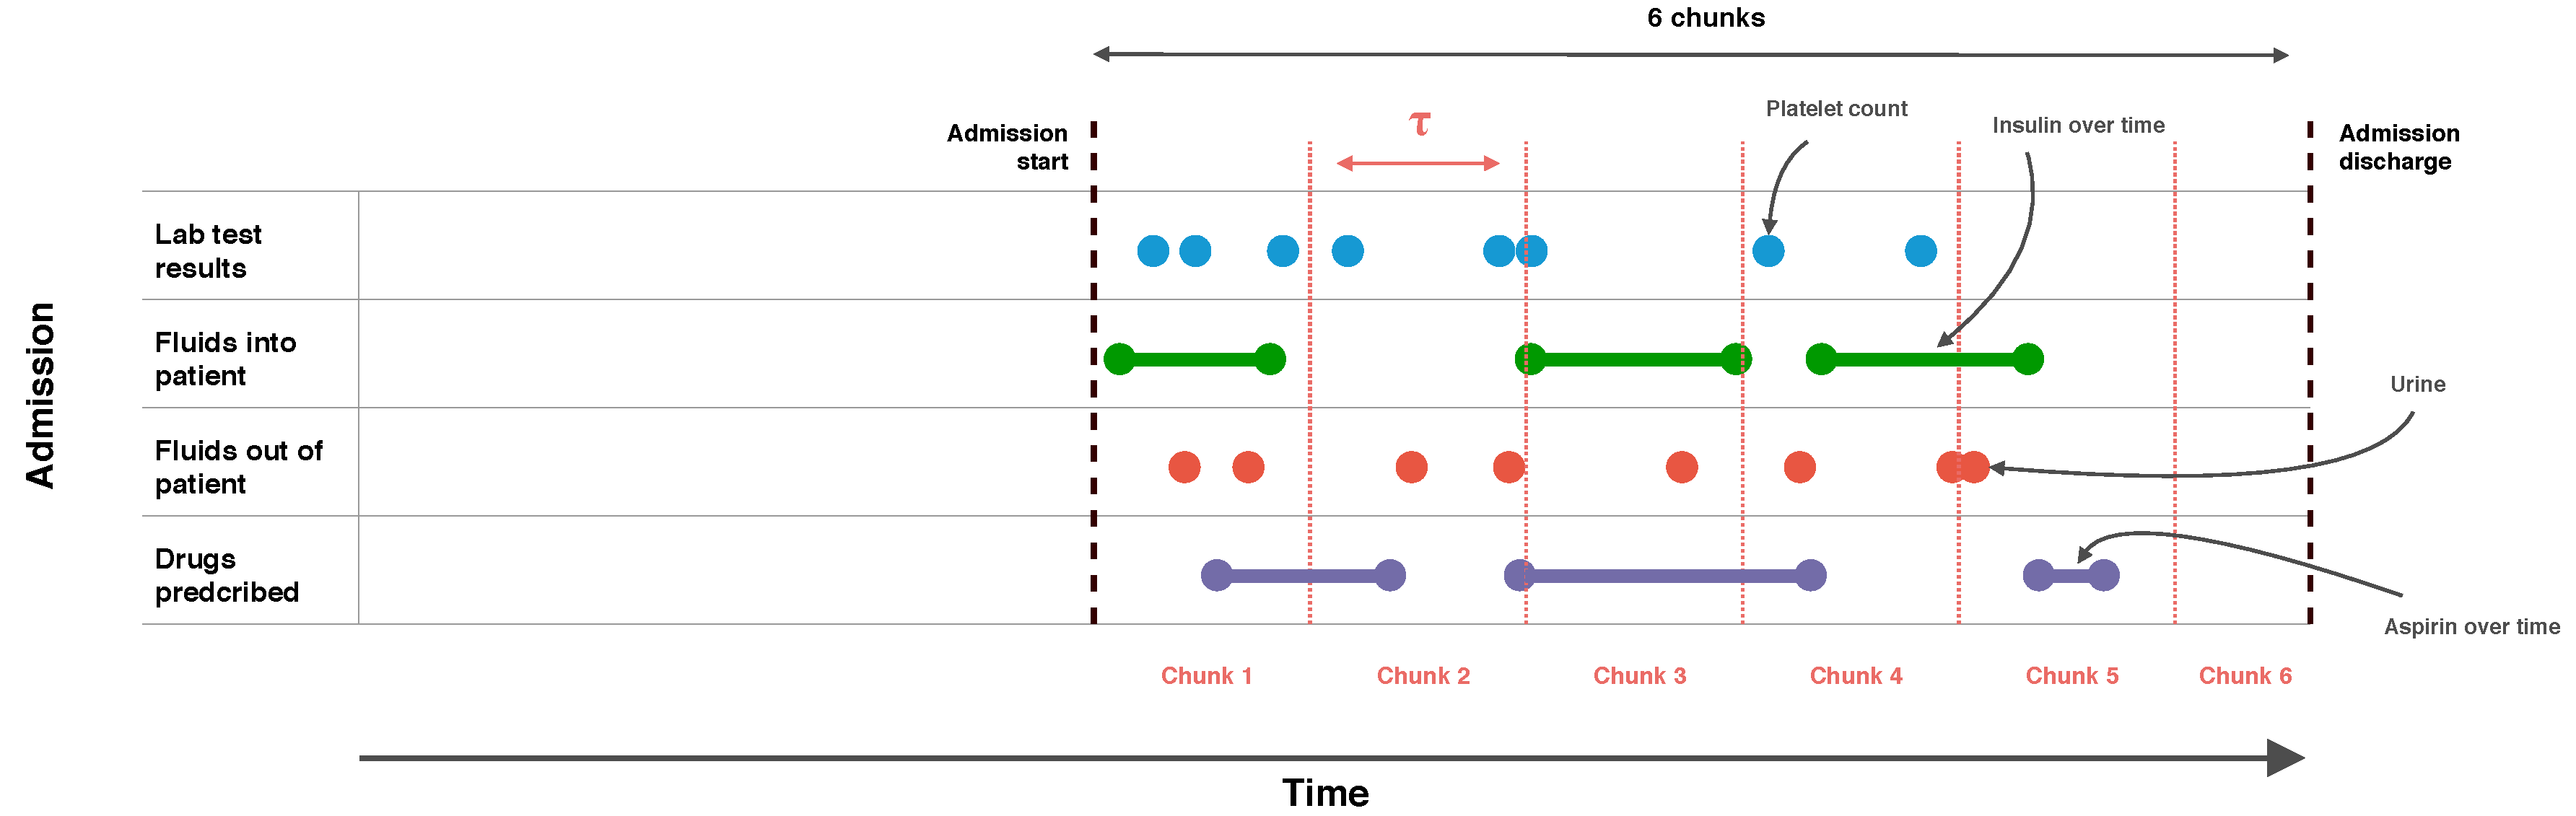
\includegraphics{figures/adm-before.pdf} \\[1.2cm]
  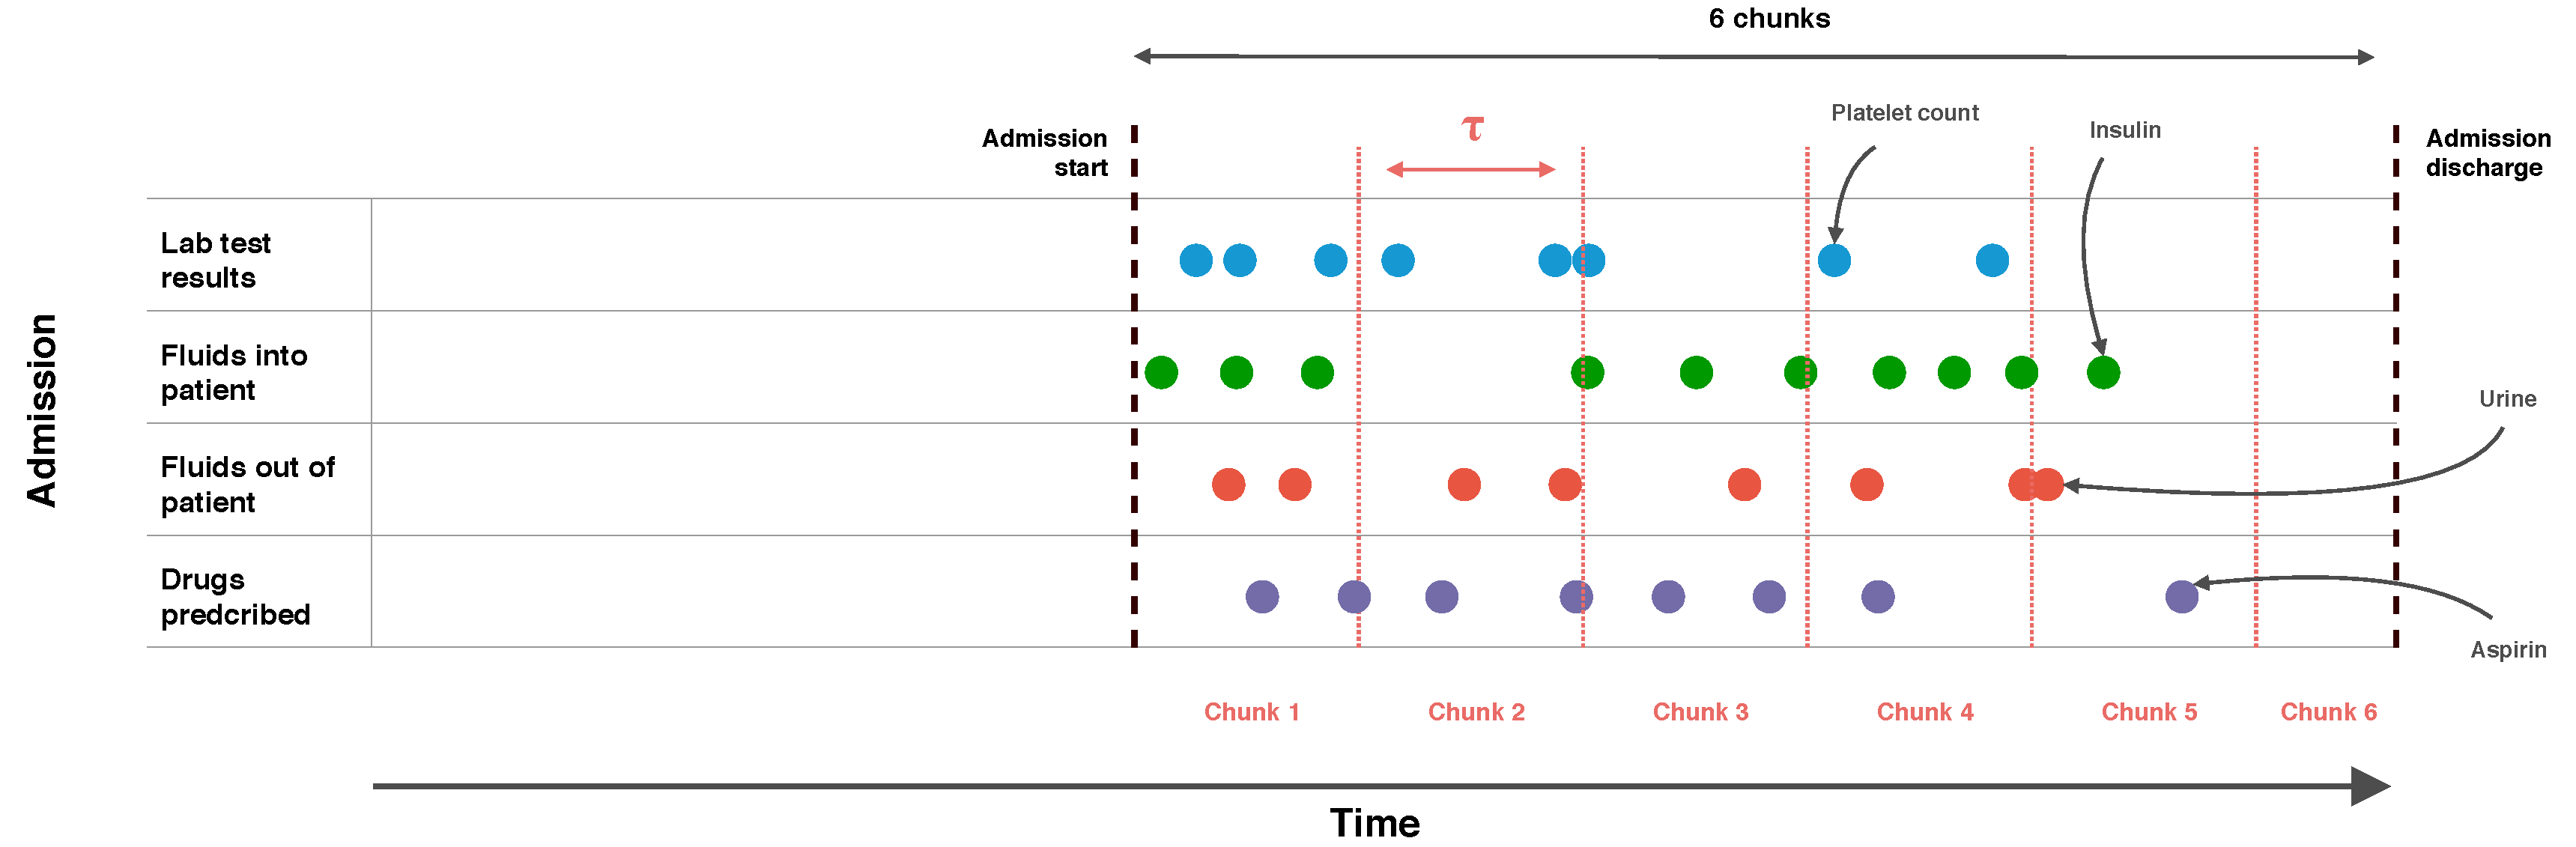
\includegraphics{figures/adm-after-1.pdf} \\[1.2cm]
  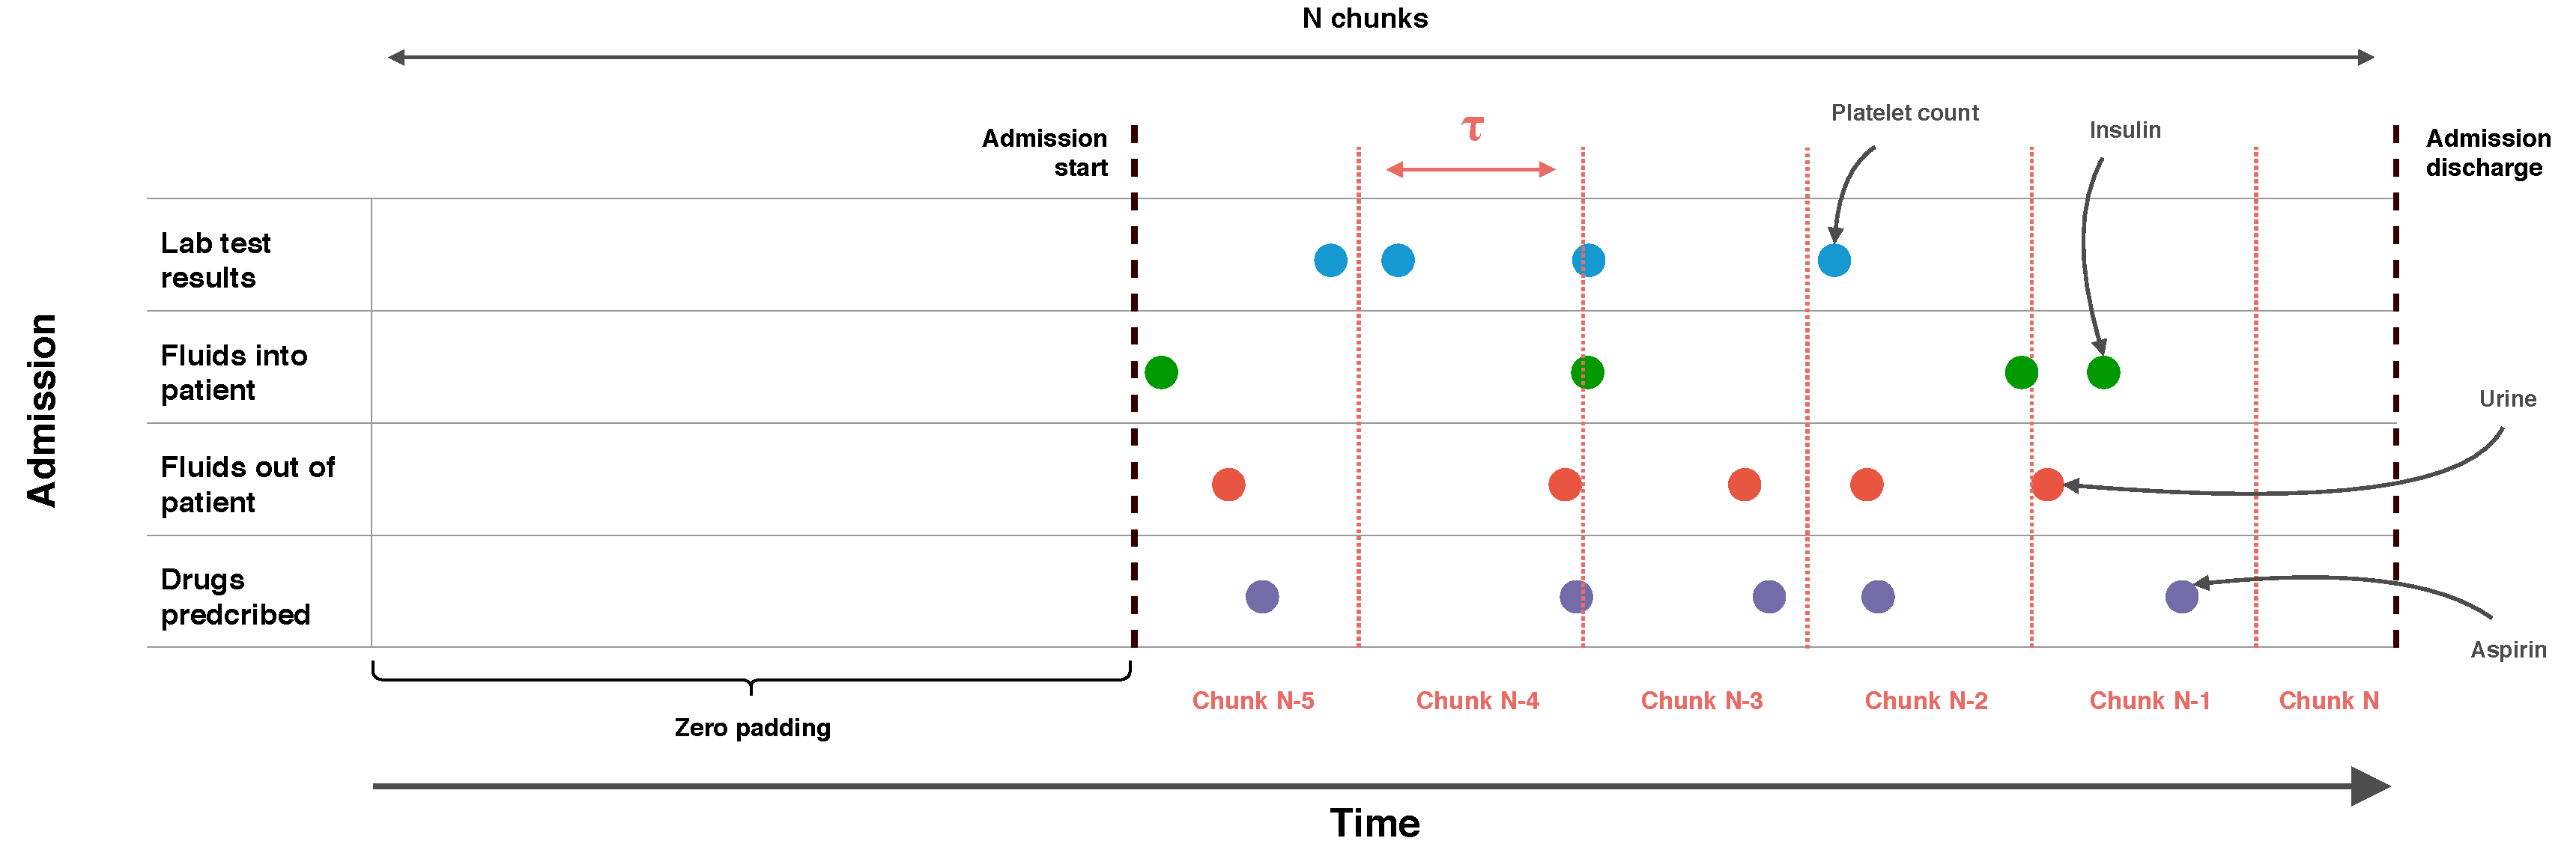
\includegraphics{figures/adm-after-2.pdf}
 \end{tabularx}
 \caption{\textbf{Top row}: The visualization of a single admission, consisting of 6 chunks of duration $\tau$, each with their respective one-time or range events. \textbf{Middle row}: The pre-processed and cleaned admission, range events have been converted to one-time events. \textbf{Bottom row}: The final version of the admission that will be fed to the downstream model. The admission is padded and events are sampled with $K=1$, thus we only have 1 event per type and per chunk of duration $\tau$. Chunks with less than $K=1$ events are also \textit{zero padded} (not shown) to match the $K$ number of events per type and per chunk.}
\end{figure}

\newpage
\section{Statistics}
\label{sec:Statistics}
This section describes the different statistics related to the data we have discussed until now, to give some quantitative metrics. In effect, the reader will be able to grasp the possibilities and distributions.

\begin{table}[H]
 \begin{center}
  \caption{Dataset size and unique values for each table}
  \begin{tabular}{| l | c | c |}
   \hline
   \textbf{Table} & \textbf{Number of events} & \textbf{Number of types} \\ \hline
   Admissions & 58'976 & - \\ \hline
   Laboratory measurements & 19'306'086 & 368 \\ \hline
   Input events CV & 11'651'110 & 2'836 \\ \hline
   Input events MV & 80'393'617 & 165 \\ \hline
   Output events & 4'217'736 & 1'113 \\ \hline
   Prescriptions & 14'728'948 & 4'465 \\ \hline
   Diagnoses & 891'142 & 9'016  \\
   \hline
  \end{tabular}
 \end{center}
\end{table}

Here are some statistics regarding each state/chunk (with $\tau=3\mbox{ hours}$) and the different events happening throughout the admission timeline:

\begin{multicols}{2}
 \centering
 \textbf{Number of chunks}
 \begin{center}
  \begin{tabular}{| l | c |}
   \hline
   \textbf{Statistic} & \textbf{Value} \\ \hline
   Minimum & 1 \\ \hline
   Maximum & 2'358 \\ \hline
   Average & 81.58 \\ \hline
   Median & 52 \\ \hline
   95th percentile & 247 \\ \hline
   99th percentile & 511 \\
   \hline
  \end{tabular}
 \end{center}\columnbreak
 \textbf{Laboratory measurements per chunk}
 \begin{center}
  \begin{tabular}{| l | c |}
   \hline
   \textbf{Statistic} & \textbf{Value} \\ \hline
   Minimum & 0 \\ \hline
   Maximum & 153 \\ \hline
   Average & 3.76 \\ \hline
   Median & 0 \\ \hline
   95th percentile & 25 \\ \hline
   99th percentile & 37 \\
   \hline
  \end{tabular}
 \end{center}
\end{multicols}

\begin{multicols}{2}
\centering
\textbf{Input CV events per chunk}
\begin{center}
 \begin{tabular}{| l | c |}
  \hline
  \textbf{Statistic} & \textbf{Value} \\ \hline
  Minimum & 1 \\ \hline
  Maximum & 189 \\ \hline
  Average & 2.46 \\ \hline
  Median & 0 \\ \hline
  95th percentile & 15 \\ \hline
  99th percentile & 28 \\
  \hline
 \end{tabular}
\end{center}\columnbreak
\textbf{Input MV events per chunk}
\begin{center}
 \begin{tabular}{| l | c |}
  \hline
  \textbf{Statistic} & \textbf{Value} \\ \hline
  Minimum & 0 \\ \hline
  Maximum & 36'400 \\ \hline
  Average & 15.95 \\ \hline
  Median & 0 \\ \hline
  95th percentile & 19 \\ \hline
  99th percentile & 464 \\
  \hline
 \end{tabular}
\end{center}
\end{multicols}

\begin{multicols}{2}
 \centering
 \textbf{Output events per chunk}
 \begin{center}
  \begin{tabular}{| l | c |}
   \hline
   \textbf{Statistic} & \textbf{Value} \\ \hline
   Minimum & 0 \\ \hline
   Maximum & 41 \\ \hline
   Average & 0.89 \\ \hline
   Median & 0 \\ \hline
   95th percentile & 4 \\ \hline
   99th percentile & 7 \\
   \hline
  \end{tabular}
 \end{center}\columnbreak
 \textbf{Prescriptions per chunk}
 \begin{center}
  \begin{tabular}{| l | c |}
   \hline
   \textbf{Statistic} & \textbf{Value} \\ \hline
   Minimum & 0 \\ \hline
   Maximum & 7'321 \\ \hline
   Average & 1.75 \\ \hline
   Median & 0 \\ \hline
   95th percentile & 9 \\ \hline
   99th percentile & 40 \\
   \hline
  \end{tabular}
 \end{center}
\end{multicols}

These different statistics helped us define the hyper-parameters related to the padding or truncation of admissions ($N$) as well as the number of events per chunk ($K$). \\

Finally, we show some plots and histograms to enlighten the reader regarding the task at hand, which is to predict the diagnosed top 50 most frequent ICD9 codes at discharge in a multi-class multi-classification fashion:

\begin{figure}[H]
 \setkeys{Gin}{width=\linewidth}
 \begin{tabularx}{\textwidth}{XXXX}
  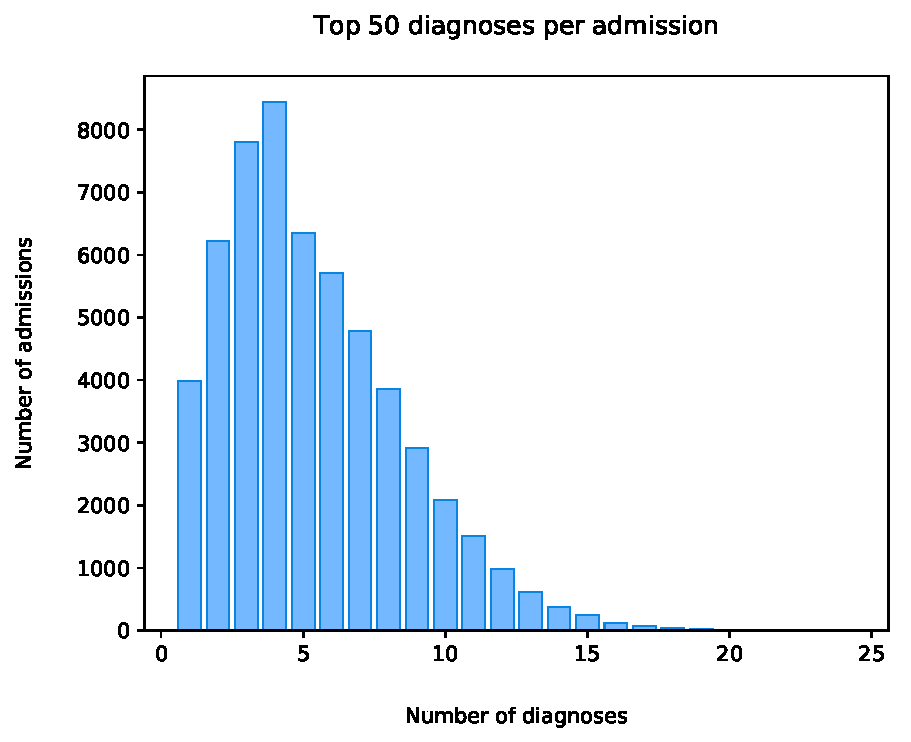
\includegraphics{figures/adm-icd9.pdf} &
  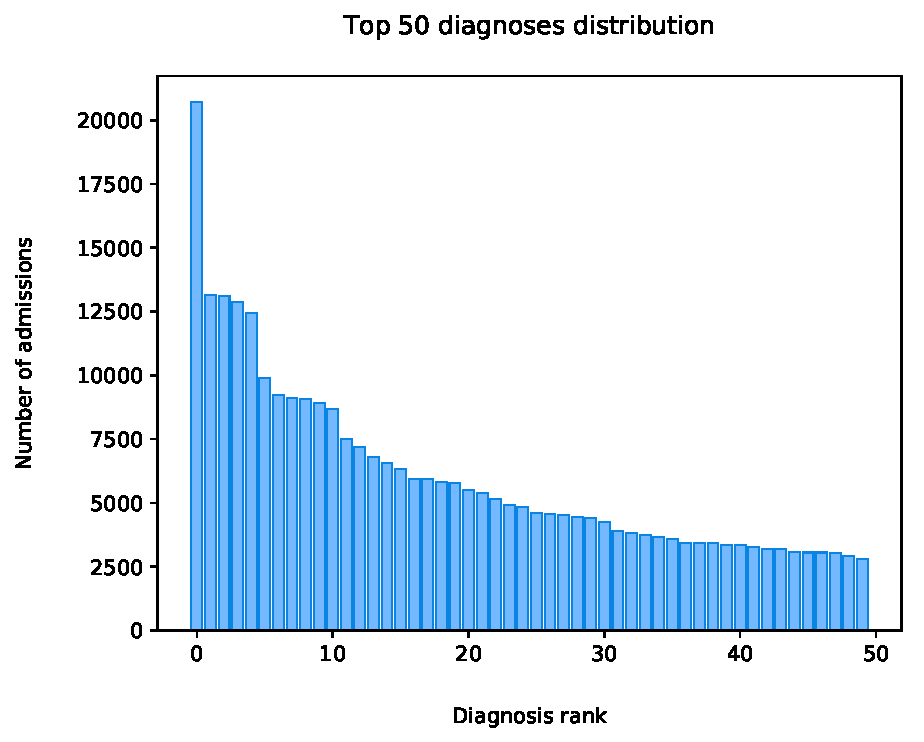
\includegraphics{figures/icd9-top50.pdf} \\
  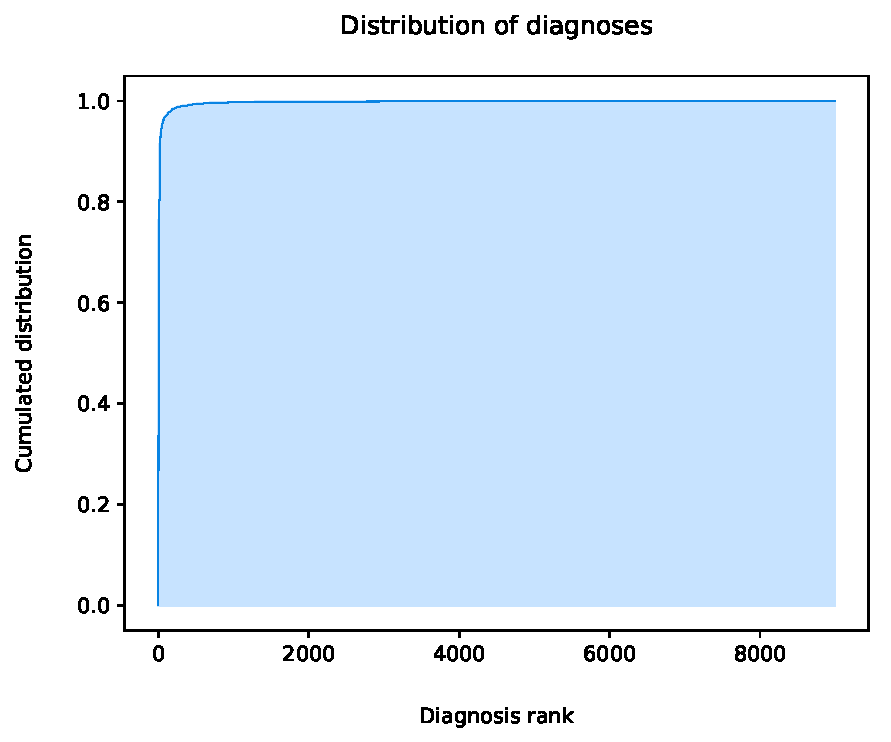
\includegraphics{figures/cdf.pdf} &
  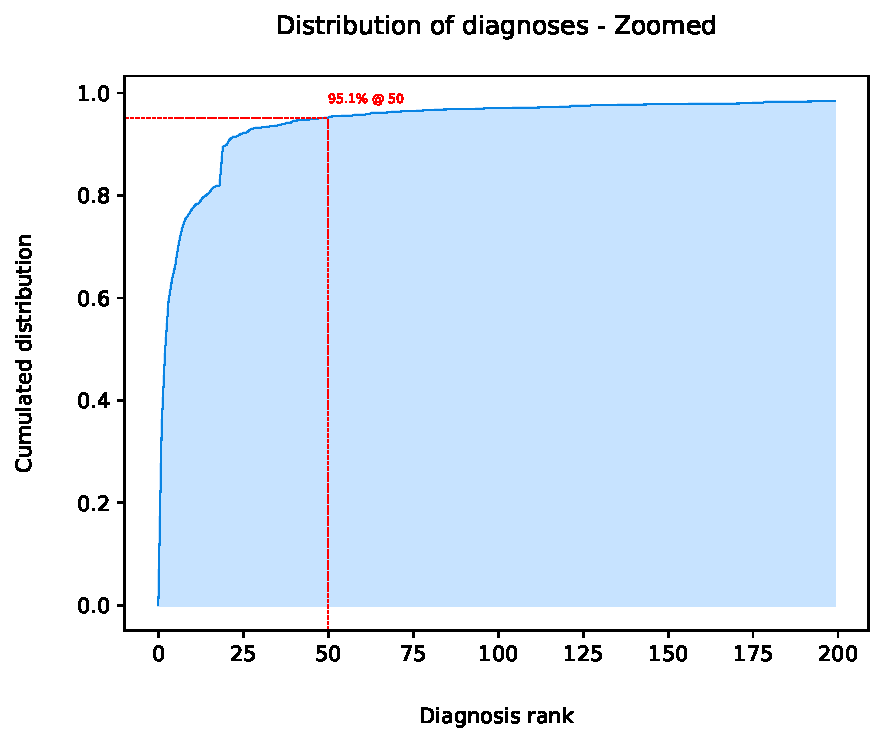
\includegraphics{figures/cdf-200.pdf} \\
 \end{tabularx}

 \caption{\textbf{Top-left}: This histogram represents the number of diagnoses per admission at discharge for the top 50 ICD 9 codes, which is interesting to bear in mind in our setup of multi-class multi-classification. \textbf{Top right}: This histogram represents the number of occurrences among the top 50 diagnoses, this is an indicator of the class imbalance or not. \textbf{Bottom-left}: The cumulative distribution of diagnoses over admissions, we can see that a few diagnoses span more than 90\% of the admissions very rapidly. \textbf{Bottom right}: The zoomed cumulative distribution of diagnoses over admissions, focusing on the top 200 most frequent diagnoses. We can see that we cover 95.1\% of admissions with the top 50 most frequent ICD9 codes.}
 \label{fig:icd9-codes}
\end{figure}